

% 2022-10-31 07:56:17  Wenbin Fan @FDU
\section{复习}
\courseTime{OCT31 2022 \\ week 7}
\chat{
上午好。

上周习题课怎么样,还有啥问题吗?

第五周讲了二维环和三维球面上的运动。上周的课程是在为本周准备,本周要讲氢原子,本质上势函数是球谐函数,类似三维球面上的运动,因此三维球面上的坐标可以辅助氢原子的求解。
}

二维环上的运动,坐标 $r,\theta$,势能
\begin{align}
    V(x,y) = V(r,\theta) = \begin{cases}
        0, \quad &r=R,\\
        \infty, \quad &r\neq R,
    \end{cases}
\end{align}
在三维极坐标下,
最大的不同是角度 $\theta$ 定义不同,势函数定义为
\begin{align}
    V(x,y,z) = V(r,\theta,\varphi) = \begin{cases}
        0,\quad &r=R,\\
        \infty, \quad &r\neq R,
    \end{cases}
\end{align}
只有当 $r=R$ 时势能为 0。

\chat{
只有做了极坐标的变换,才能通过变换哈密顿量求解。

我们这个宇宙挺惨的,只能求解分离变量的二维系统。人们做了很多的尝试,即如何坐标变换使得系统分离坐标。哪怕是两个变量,也无法解析解。
}

二维环的极坐标表述,
\begin{align}
    \hat H = - \frac{\hbar^2}{2m} \left(
        \pdv[2]{r} + \frac1r \pdv{r} + \frac1{r^2} \pdv[2]{\theta}
    \right)
\end{align}
在笛卡尔空间中的表述,
\begin{align}
    \hat H = -\frac{\hbar^2}{2m} \left(
        \pdv[2]{x} + \pdv[2]{y}
    \right)
\end{align}
通常会写成劈形算符 $\nabla$ nabla 的形式,
\begin{align}
    \hat H = -\frac{\hbar^2}{2m} \hat \nabla^2
\end{align}

三维球面的势能,类似地有
\begin{align}
    \hat H = - \frac{\hbar^2}{2m} \left(
        \pdv[2]{r} + \frac1r \pdv{r} + \frac1{r^2} \hat\Lambda^2(\theta,\varphi)
    \right), 
\end{align}
\chat{
二维、三维的差别在于角度部分的算符,径向部分是一样的。

二维和三维的不同,是环和面的区别。利用径向部分不变的条件,可以将哈密顿量简化。
}
二维环上的粒子,
\begin{align}
    \hat H = - \frac{\hbar^2}{2m} \frac1{R^2} \pdv[2]{\theta} = - \frac{\hbar^2}{2I} \pdv[2]{\theta}, \label{eq:2d_ring_h_simp_rev}
\end{align}
只剩下角度部分。求解得到通解
\begin{align}
    \phi(\theta) = A \ee^{\ii m\theta} + B \ee^{-\ii m \theta},\label{eq:2d_ring_h_general_sol_rev}
\end{align}
其中 $M$ 是需要量子化的,同时发现这个通解是哈密顿方程 \eqref{eq:2d_ring_h_simp_rev} 的本征解,
写出 $l_z$,
\begin{align}
    \hat l_z = - \ii\hbar \left(
        x \pdv{y} - y \pdv{x}
    \right) = -\ii\hbar \pdv{z}
\end{align}
发现 \eqref{eq:2d_ring_h_general_sol_rev} 并不是 $l_z$ 的本征解。但是,环和面上的粒子的 $\hat l_z$ 是互易的,有共同的本征函数解,
% 【等价的】但 lz 来说不是等价的,【找到一套解】
% 还是不太明白 % 2022-10-31 11:13:49  Wenbin Fan @FDU
\begin{align}
    \phi(\theta) = A\ee^{\ii m \theta}, m = 0,\pm1,\pm2,\cdots
\end{align}
通量的右手螺旋定则,从经典来说这肯定与磁性相关,所以 $m$ 是磁量子数。

对于三维球面,利用径向为常数的条件,哈密顿量
\begin{align}
    \hat H = -\frac{\hbar^2}{2m} \frac1{R^2} \hat \Lambda^2 = - \frac{\hbar^2}{2I} \hat \Lambda^2,
\end{align}
解出来
\begin{align}
    \hat H Y(\theta, \varphi) = E Y(\theta, \varphi)
\end{align}
把角度部分写成各部分变量的乘积,即分离变量,得到关于 $\varphi$ 的部分
\begin{align}
    \pdv[2]{\Phi(\varphi)}{\varphi} = - m^2 \Phi(\varphi), 
\end{align}
解得
\begin{align}
    \Phi(\varphi) = \frac1{\sqrt{2\pi}} \ee^{\ii m \varphi}, \quad m = 0,\pm1, \pm2, \cdots,
\end{align}
这与二维环的角度部分的解是一致的。$\theta$ 部分更复杂,满足
\begin{align}
    \sin^2\theta \pdv[2]{\Theta(\theta)}{\theta} + \sin\theta\, \cos\theta \pdv{\Theta(\theta)}{\theta} = (m-M^2 \sin\theta) \Theta(\theta),
\end{align}
由此可知 $M$ 的量子化条件是 $M^2 = l(l+1)$,
\begin{align}
    &|m| = l - k, \quad k = 0,1,2,\cdots,
    \\
    &m = 0, \pm1, \pm2, \cdots
\end{align}
反过来由 $l$ 定义 $M$ 更方便一些,$M$ 必然不会小于 $l$,做变换
\begin{align}
    \begin{pmatrix}
        m \\ M
    \end{pmatrix}
    \rightarrow
    \begin{pmatrix}
        m_l \\ l
    \end{pmatrix},
\end{align}
得到能量为
\begin{align}
    E = - \frac{\hbar^2}{2I} l(l+1),
\end{align}
% 角度部分为
% \begin{align}
%     Y(\theta,\phi) = \sum_{135,246[][]}
% \end{align}
% 没拍全
这就是上一部分的内容。

\chat{
有同学问 Morse 势的推导不太清楚,实际上在量化里的很多推导都是在用数学物理方法中著名的结论,我们要做的就是如何利用已有的结论。级数展开是最简单的求解方法,是万能的,还可以得到量子化条件。
}
\section{常见的二阶常微分方程}
再介绍一下什么是二阶常微分方程,
\begin{align}
    y''(x) + P(x) y'(x) + Q(x) y = 0,
\end{align}
更常见的形式是二阶项的系数不为 1,
\begin{align}
    P(x) y''(x) + Q(x) y'(x) + R(x) y = 0,
\end{align}
由幂级数展开,
\begin{align}
    y = \sum_{k=0}^\infty = a_k x^k 
\end{align}
并得到 $y'$、$y''$,以及 $a_k$ 的递推关系,
\begin{align}
    a_k = c_1 a_{k-1} + c_2 a_{k-2} + \cdots + c_{k-1} a_1 + c_k a_0.
\end{align}

再列几个二阶线性微分方程,
\begin{align}
    y'' - 2x y' + 2ny =0,
\end{align}
这是求解谐振子时用到的微分方程,即 Hermite 微分方程。
\begin{align}
    (1-x^2) y'' - 2x y' + l(l+1) y = 0,
\end{align}
这是勒让德方程。
\begin{align}
    (1-x^2) y'' - 2x y' + \left[
        l(l+1) - \frac{m^2}{1-\lambda^2}
    \right] y = 0
\end{align}
连带勒让德方程。
\begin{align}
    x y'' + (1-x) y' + \nu y = 0,
\end{align}
拉盖尔方程,
\begin{align}
    x y'' + (a+1 - x)y' + \nu y = 0,
\end{align}
连带拉盖尔方程,在一阶项里多了常数,而连带勒让德方程实在 0 阶项里多了常数。
\begin{align}
    x^2 y'' + x y' + (x^2 - n^2) y = 0,
\end{align}
贝塞尔方程,
\begin{align}
    x(1-x) y'' + [r - (\alpha + \beta + 1)x] y' - \alpha \beta y =0
\end{align}
称作超几何方程。

\chat{
我们可以看到,能求解的二阶微分方程并不多,被冠名的也就这么几个。在流体力学等领域,人们求解出了许多方程,后来发现也可应用在波动力学领域。

有了这些知识,这周就开始求解氢原子。
}

\chapter{氢原子及类氢原子体系}

\chat{
每周学的内容都在逼近真实体系。从数学角度,氢原子复杂在哪里?首先是势能更复杂,其次,氢原子是个二体系统。
}
我们从单粒子拓展到了双粒子体系。
% 电子 $m_1$、$(x_1, y_1, z_1)$、$-e$,【列表格】
\begin{table}[ht]
\centering
% \caption{Thicker horizontal lines above and below the table.}
\begin{tabular}[t]{lcc}
\toprule
&原子核 & 电子 \\
\midrule
质量 & $m_2$ & $m_1$ \\
坐标 & $(x_2,y_2,z_2)$ & $(x_1,y_1,z_1)$\\
电荷 & $+e$ & $-e$ \\
\bottomrule
\end{tabular}
\end{table}%

\begin{figure}[tp]\centering
    \begin{tikzpicture}[scale=1.0]
        % axis
        \draw[->] (-0.5,0) -- (3, 0);
        \draw[->] (0,-0.5) -- (0, 3);
        \draw[->] (0.353, 0.353) -- (-1.4, -1.4);
    
        \fill[blue] (2,-0.5) circle (0.05);
        \fill[blue] (1, 2) circle (0.05);
        \draw[->, thick] (0,0) -- (2, -0.5);
        \draw[->, thick] (0,0) -- (1, 2);
    
        \node[right] at (1,2) {$\vec r_1 = (x_1, y_1, z_1)$};
        \node[right] at (2,-0.5) {$\vec r_2 = (x_2, y_2, z_2)$};
    
    \end{tikzpicture}
    \caption{两体示意图}
    \end{figure}
% 2022-10-31 08:40:40  Wenbin Fan @FDU
设二者的坐标
\begin{align}
    &\vec r_1 = x_1 \vec i + y_1 \vec j + z_1 \vec k, \\
    &\vec r_2 = x_2 \vec i + y_2 \vec j + z_2 \vec k,
\end{align}
因此二者之间距离
\begin{align}
    \vec r &= \vec r_2 - \vec r_1 \\
    &= (x_2 - x_1) \vec i + (y_2 - y_1) \vec j + (z_2 - z_1) \vec k\\
    &=x \vec i + y \vec j + z \vec k,
\end{align}
引入了没有下标的坐标。

原子核和电子之间的力是库伦相互作用,
\begin{align}
    F = \frac{|e\times(-e)|}{r^2} = \frac{e^2}{r^2},
\end{align}
保守力(与路径无关的力)的势能为
\begin{align}
    V(r) = \int_r^\infty \frac{e^2}{r^2} \dd r = - \frac{e}{r},
\end{align}
对于氢原子,势能 $V(r) = -\frac{e^2}{r}$,类氢离子 $V(r) = - \frac{Z \ee^2}{r}$,其中 $Z$ 是核电荷数。

哈密顿算符
\begin{align}
    \hat H &= \hat T + \hat V \\
    &= -\frac{\hbar^2}{2m_1} \left(
        \pdv[2]{x_1} + \pdv[2]{y_1} + \pdv[2]{z_1}
    \right) 
    - \frac{\hbar^2}{2m_2} \left(
        \pdv[2]{x_2} + \pdv[2]{y_2} + \pdv[2]{z_2}
    \right) \notag\\
    &\phantom{=} + V\left(
        |\vec r_1 - \vec r_2|
        \right)
\end{align}
% 2022-10-31 08:54:24  Wenbin Fan @FDU
\courseTime{2 of 4, week 7}
将哈密顿量作用到波函数上
\begin{align}
    \hat H \psi(\vec r_2, \vec r_1) = E \psi (\vec r_2, \vec r_1)
\end{align}
\chat{
只有可分离的两个变量才可以求解,希望可以分离变量。尝试坐标变换,将两个坐标变换成一个坐标,那么有可能求解。
}
考虑质心坐标,这是个很自然的拓展,想到这一步应该不难。质心坐标
\begin{align}
    \vec R = (X,Y,Z) = X \vec i + Y \vec j + Z \vec k,
\end{align}
那么坐标可表示为
\begin{align}
    X = \frac{m_1 x_1 + m_2 x_2}{M}, \quad Y = \frac{m_1 y_1 + m_2 y_2}{M}, \quad
    Z = \frac{m_1 z_1 + m_2 z_2}{M}
\end{align}
其中 $M = m_1 + m_2$。如果 $m_1 = m_2$,质心坐标便是平均坐标。相对坐标
\begin{align}
    \vec r = (x,y,z) = x \vec i + y \vec j + z \vec k,
\end{align}
其中分量为
\begin{align}
    x = x_2 - x_1, \quad y = y_2 - y_1, \quad z= z_2-z_1,
\end{align}
做变量代换
\begin{align}
    \begin{cases}
        x_1, y_1, z_1\\
        x_2, y_2, z_2
    \end{cases}
    \Rightarrow 
    \begin{cases}
        X,Y,Z\\
        x,y,z
    \end{cases}
\end{align}
% 【讨论】
变换成质心运动和相对运动。

坐标偏导
\begin{align}
    &\pdv{\psi}{x_1} = \pdv{\psi}{X} \pdv{X}{x_1} + \pdv{\psi}{x}\pdv{x_1}{x} =
    \left(\frac{m_1}{M} \pdv{x} - \pdv{x}\right)\psi, \\
    &\pdv[2]{\psi}{x_1} = 
    \left[
        \left(\frac {m_1}M\right)^2 \pdv[2]{X} - \frac{2m_1}{M} \pdv[2]{}{X}{x} + \pdv[2]{x}
    \right]\psi,
    \\
    &\pdv[2]{\psi}{x_2} = 
    \left[
        \left(\frac {m_2}M\right)^2 \pdv[2]{X} + \frac{2m_2}{M} \pdv[2]{}{X}{x} + \pdv[2]{x}
    \right]\psi,
\end{align}
同理由 $y$ 的坐标偏导
\begin{align}
    &\pdv[2]{\psi}{y_1} = 
    \left[
        \left(\frac {m_1}M\right)^2 \pdv[2]{Y} - \frac{2m_1}{M} \pdv[2]{}{Y}{y} + \pdv[2]{y}
    \right]\psi,
    \\
    &\pdv[2]{\psi}{y_2} = 
    \left[
        \left(\frac {m_2}M\right)^2 \pdv[2]{Y} + \frac{2m_2}{M} \pdv[2]{}{Y}{y} + \pdv[2]{y}
    \right]\psi,
\end{align}
\begin{align}
    &\pdv[2]{\psi}{z_1} = 
    \left[
        \left(\frac {m_1}M\right)^2 \pdv[2]{Z} - \frac{2m_1}{M} \pdv[2]{}{Z}{z} + \pdv[2]{z}
    \right]\psi,
    \\
    &\pdv[2]{\psi}{z_2} = 
    \left[
        \left(\frac {m_2}M\right)^2 \pdv[2]{Z} + \frac{2m_2}{M} \pdv[2]{}{Z}{z} + \pdv[2]{z}
    \right]\psi,
\end{align}
对于动能算符,最重要的是,我们希望变换到质心坐标
\begin{align}
    \frac1{m_1} \hat \nabla_2^2 + \frac1{m_2} \hat \nabla_2^2  = \frac1M \hat \nabla_M + \frac1{\mu} \hat \nabla_\mu,
\end{align}

合并含有 $M$ 的项,
\begin{multline}
    \frac 1{m_1} 
    \left(\frac{m_1}M\right)^2
    \left(
        \pdv[2]{X} + \pdv[2]{Y} + \pdv[2]{Z}
    \right) 
    + \frac1{m_2} 
    \left(\frac{m_2}M\right)^2 
    \left(
        \pdv[2]{X} + \pdv[2]{Y} + \pdv[2]{Z}
    \right) \\
     = \frac{m_1 + m_2}{M} \left(
        \pdv[2]{X} + \pdv[2]{Y} + \pdv[2]{Z}
     \right) = \frac1M \hat \nabla_M^2,
\end{multline}

以上二阶偏导中的第二项,除以各自质量后,耦合项全部相加抵消了。

合并二阶偏导中的第三项,
\begin{multline}
    \frac1{m_1} \left(\pdv[2]x + \pdv[2]y + \pdv[2]z\right) +
    \frac1{m_2} \left(\pdv[2]x + \pdv[2]y + \pdv[2]z\right) \\
    = \frac{m_1 + m_2}{m_1 m_2} \left(
        \pdv[2]x + \pdv[2]y + \pdv[2]z
    \right) = \frac{1}{\mu} \hat \nabla_\mu,
\end{multline}
这里正式引入了\boldtext{折合质量},
\begin{align}
    \mu = \frac{m_1m_2}{m_1 + m_2}, \quad \frac1{\mu}=\frac1{m_1} + \frac1{m_2}. 
\end{align}
氢原子的折合质量
\begin{align}
    \mu_{\mathrm H} = \frac{m_{\mathrm e} m_{\mathrm e}}{m_{\mathrm e}+m_{\mathrm e}} = \frac {m_{\mathrm e}} {1 + \frac{m_{\mathrm e}}{m_{\mathrm p}}} = \frac{m_{\mathrm e}}{1 + \num{5.45E-4}} = \num{0.99946} \,m_{\mathrm e}, 
\end{align}
通过折合质量,分离了整体运动和相对运动。因为原子核和电子的质量相差 3 个数量级,$1 \,m_{\mathrm p} = 1836 \,m_{\mathrm e}$。

重新写哈密顿算符,
\begin{align}
    \hat H &= \frac{\hat p_1^2}{2m_1} + \frac{\hat p_2^2}{2m_2} + V (|\vec r_1 - \vec r_2 |) \\
    &= \frac{\hat p_M^2}{2M} + \frac{\hat p_m^2}{2m} + V(x,y,z)
    \label{eq:hydro_cent_h}
\end{align}

\suppInfo{偏导数}{
还需要讲一点,变量代换后的偏导,
\begin{align}
    F(x,y) = F(f_1,f_2), \quad f_1=f_1(x,y), f_2=f_2(x,y),
\end{align}
其中的偏导
\begin{align}
    \pdv{F}{x} &= \left(\pdv{F}{f_1}\right)_{f_2} 
    \left[
        \left(\pdv{f_1}{x}\right)_y \pdv{x}{x}
        + \left(\pdv{f_1}{y}\right)_x \pdv{y}{x}
    \right] \notag\\
    &\phantom{=}
    +
    \left(\pdv{F}{f_2}\right)_{f_1}
    \left[
        \left(\pdv{f_2}{x}\right)_y \pdv{x}{x}
        + \left(\pdv{f_2}{y}\right)_x \pdv{y}{x}
    \right] 
\end{align}
如果 $x,y$ 线性无关,那么 $\pdv{y}{x} = 0$、$\pdv{x}{x} = 1$。
}
\chat{
在求上面一系列二阶偏导的时候,我们不加证明地利用了
\begin{align}
    \pdv{x_1} \pdv{\psi}{X} = \pdv{X} \pdv{\psi}{x_1},
\end{align}
实际上背后隐藏的是
\begin{align}
    &\left[
        \pdv{x_1}, \pdv{X}
    \right] = 0, \\
    & [\hat \nabla_1, \hat \nabla\!_M] = 0,\\
    &[\hat \nabla_1, \hat \nabla\!_\mu] = 0,
\end{align}
}

当哈密顿量写成质心和相对运动时,\eqref{eq:hydro_cent_h} 继续写成
\begin{align}
    \hat H = -\frac{\hbar^2}{2m} \hat \nabla_M^2 -
    -\frac{\hbar^2}{2m} \hat \nabla_\mu^2 + V(r),
\end{align}
相对运动包含了相互作用势能。

% 与之前有什么不一样?【】【】
% 2022-10-31 09:29:46  Wenbin Fan @FDU
\chat{
很多内容需要深入思考。本课是物化的扩展,更深入地讲解理论知识。希望本课的推导,能帮助同学们理解知识点。
}

\section{中心力场}
这是一个\boldtext{中心力场}的问题,
\begin{align}
    \psi_{\mathrm{tot}} = \psi_{\mathrm{tr}}(x,y,z) \,\psi_(x,y,z),
\end{align}
可以天然地分离成整体和相对运动的波函数,将其代入薛定谔方程,
\begin{align}
    \left[
        -\frac{\hbar^2}{2M}\hat\nabla_M^2 - \frac{\hbar^2}{2m} \hat\nabla_\mu^2 + V(r) 
    \right] \psi_{\mathrm{tr}} \psi = E \psi_{\mathrm{tr}} \psi
\end{align}
整理得到
\begin{align}
    - \frac{\hbar^2}{2M}\hat\nabla_M^2 \psi_{\mathrm{tr}} = \psi_{\mathrm{tr}} \left[
        E + \frac{\hbar^2}{2\mu}\hat\nabla_\mu^2 - V(r)
    \right]\psi
\end{align}
两边同时除以整体波函数
\begin{align}
    -\frac{\hbar^2}{2m} \frac1{\psi_{\mathrm{tr}}} \hat\nabla_M^2 \psi_{\mathrm{tr}} = \frac1{\psi} \left[
        E + \frac{\hbar^2}{2\mu}\hat\nabla_\mu^2 - V(r)
    \right]\psi
\end{align}
左边只与整体运动有关,右边只与相对运动有关,因此波函数可以分成两部分,
\begin{align}
    & - \frac{\hbar^2}{2m} \hat \nabla_m \psi_{\mathrm{tr}} = E_\mathrm{tr} \psi_{\mathrm{tr}}, 
    \label{eq:hydro_Htr}
    \\
    & \left[-\frac{\hbar^2}{2m} \hat\nabla_\mu^2 + V(x,y,z)\right] \psi = E_\mathrm{int} \psi
    \label{eq:hydro_Hint}
    角度部分\end{align}
其中,系统整体能量 $E = E_{\mathrm{tr}} + E_{\mathrm{int}}$。平动能 $E_{\mathrm{tr}}$ 用 $K$ 表示,便于后面写。

平动的求解,类比自由粒子,
\begin{align}
    -\frac{\hbar^2}{2m} \hat\nabla_\mu^2 \psi + V(x,y,z) \psi = E_\mathrm{int} \psi, 
\end{align}

\homework{\textbf{7.1}  对于3个粒子的体系,约化质量后的 $\hat H$ 能否分离变量,$N$ 个粒子呢?为什么要引入 Born--Oppenheimer 近似?}
举个简单的粒子,三粒子可以用 He 原子或氢分子离子来理解,那么能否分离变量呢?下午讲。

\courseTime{OCT31 2022 下午}
动能算符
\begin{align}
     \hat \nabla^2_\mu = \pdv[2]x + \pdv[2]y + \pdv[2]z = \pdv[2]r + \frac2r \pdv{r} - \frac1{\hbar^2r^2} \hat L^2 (\theta, \psi), 
\end{align}
其中
\begin{align}
    \hat L^2 = -\hbar^2 \left(
        \frac1{\sin^2\theta} \pdv[2]{\psi} + \cot\theta \pdv{\theta} + \pdv[2]\theta
    \right). 
\end{align}
上周已经求了
\begin{align}
    \hat L^2 Y_l^{m_l} = \hbar^2 \,l(l+1) Y_l^{m_l}(\theta,\varphi), 
\end{align}
【】
设
\begin{align}
    \Phi(r,\theta,\varphi) = R(r) Y_l^{m_l} (\theta,\varphi),
\end{align}
提出与角度无关的部分
\begin{multline}
    -\frac{\hbar^2}{2m} 
    \left[
    Y_l^{m_l} (\theta,\varphi) \left(\pdv[2]r + \frac2r \pdv{r}\right) R(r) - \frac{R(r)}{\hbar^2r^2} \hat L^2 Y_l^{m_l} (\theta,\varphi)
    \right] \\
    + V(r) R(r) Y_l^{m_l} (\theta, \varphi) = E_{\mathrm {int}}\psi,
\end{multline}
两边同时除以波函数,得到
\begin{multline}
    -\frac{\hbar^2}{2m} \frac1{R(r)} 
    \left(\pdv[2]r + \frac2r \pdv{r}\right) R(r)  \\ + \frac1{2\mu r^2} \frac1{Y_l^{m_l}(\theta,\varphi)} \hat L^2 \frac1{Y_l^{m_l}(\theta,\varphi)}  = E_{\mathrm{int}} - V(r)
\end{multline}
第一项与角度无关,但是第二项里有个 $\frac1{r^2}$,争取把第二项变成与 $r$ 无关的项。继续化简,
\begin{align}
    &\text{LHS} = -\frac{\hbar^2}{2m} \frac{r^2}{R(r)} 
    \left(\pdv[2]r + \frac2r \pdv{r}\right) R(r) - (E_{\mathrm{int}} - V(r)) r^2, \\
    &\text{RHS} = -\frac1{2\mu} \frac1{Y_l^{m_l}} \hat L^2 Y_l^{m_l}(\theta,\varphi),
\end{align}
左边与径向有关,右边与角度有关,因此二者都等于常数 $\text{LHS} = \text{RHS} = K$。

角度相关项,
\begin{align}
    \hat L^2 Y_l^{m_l} (\theta,\varphi) &= 2 \mu K Y_l^{m_l} (\theta,\varphi) \\
    &= \hbar^2 \,l(l+1) Y_l^{m_l} (\theta,\varphi),
\end{align}
解出来
\begin{align}
    K = - \frac{\hbar^2 l(l+1)}{2\mu},
\end{align}
那么把 $K$ 代回径向部分,
\begin{align}
    -\frac{\hbar^2}{2\mu} r^2 \left(\pdv[2]r + \frac2r \pdv{r}\right) R(r) - [ E_{\mathrm{int}} - V(r)] r^2 R(r) = 
    - \frac{\hbar^2 l(l+1)}{2\mu} R(r)
\end{align}
把左边的 $r^2$ 除到右边去,整理可得
% 2022-10-31 13:46:43  Wenbin Fan @FDU
% 随时可以提问
\begin{align}
    -\frac{\hbar^2}{2\mu} \left(\pdv[2]r + \frac2r \pdv{r}\right) R(r)
    + \left[
        \frac{\hbar^2 l(l+1)}{2\mu} + V(r)
    \right] R(r)
    = 
    E_{\mathrm{int}} R(r),
\end{align}
我们更偏好最高阶项没有系数,
\begin{align}
    \left(\pdv[2]r + \frac2r \pdv{r}\right) R(r) 
    + \left\{
        - \frac{l(l+1)}{r^2} + \frac{2\mu}{\hbar^2} 
        \left[
            E_{\mathrm{int}} - V(r)
        \right] 
    \right\} R(r) = 0,
\end{align}

\section{径向部分的求解}
\begin{figure}[tp]\centering
    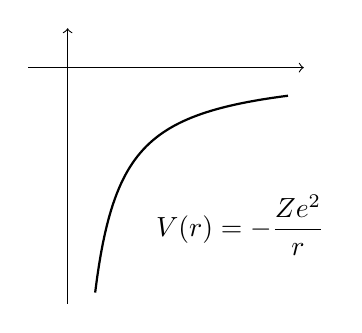
\begin{tikzpicture}[scale=1.0]
        % axis
        \draw[->] (-0.5,0) -- (3, 0);
        \draw[->] (0,-3) -- (0, 0.5);
    
        \draw[domain=0.35:2.8,thick,samples=100] plot (\x,{-1/\x});
        \node[right] at (1,-2) {$V(r) = -\displaystyle\frac{Ze^2}{r}$};
    
    \end{tikzpicture}
    \caption{氢原子中的吸引势}
    \label{fig:H_attraction}
    \end{figure}
势函数如图 \ref{fig:H_attraction}。当两体接近时,势能趋于 $-\infty$。如果能量 $E>0$ 表示 $T>0>V$,解离态。只有当能量 $E<0$ 才表示束缚态,仅考虑这种情况。

上面方程里的系数太多了,做变量代换,目的是为了凑成已知的微分方程。令
\begin{align}
    a^2 = -\frac{2\mu E_{\mathrm{int}}}{\hbar^2}, \quad 
    a = \frac{\sqrt{2\mu E_{\mathrm{int}}}} {\hbar}, 
\end{align}
那么从 $E$ 的量子化,变成了 $a$ 的量子化,重写方程,
\begin{align}
    R''(r) + \frac2r R'(r) + \left[
        -a^2 + \frac{2\mu}{\hbar^2} \frac{Ze^2}{r} - \frac{l(l+1)}{r^2}
    \right] R(r) = 0, \label{eq:hydro_quantized_a}
\end{align}
我们不喜欢中括号中间一项,如果有它,方程的解会变得很复杂。利用\boldtext{坐标缩放},尝试消去它。定义 $\rho = kr$,接下来推导 $k$ 为何值时可以消去。则 $R(r) = R(\rho)$,偏导为
\begin{align}
    \pdv{R(\rho)}{r} = \pdv{R(\rho)}{\rho} \pdv{\rho}{r} = k \pdv{R(\rho)}{\rho}, \quad \pdv[2]{R(\rho)}{r} 
    = k^2 \pdv[2]{R(\rho)}{\rho}
\end{align}
\begin{lstlisting}
D[R[k r], {r, 2}] /. {r -> \[Rho]/k}
>> k^2 (R^\[Prime]\[Prime])[\[Rho]]
\end{lstlisting}
那么 \eqref{eq:hydro_quantized_a} 变换成了
\begin{align}
    k^2 R''(\rho) + \frac{2k}{\rho/k} R'(\rho) + \left[
        -a^2 + \frac{2\mu}{\rho} \frac{Ze^2k}{\rho} - \frac{l(l+1)k^2}{\rho^2}
    \right] R(\rho) = 0
\end{align}
约掉高次项的 $k^2$。此时注意到,当 $k=2a$ 时,有
\begin{align}
    R''(\rho) + \frac2{\rho} R'(\rho) + \left[
        \frac14 + \frac{\lambda}{\rho} - \frac{l(l+1)}{\rho^2}
    \right] R(\rho) = 0
\end{align}
现在方程就简单一些了。

按照经验,我们先求解渐近形式。当 $\rho \rightarrow \infty$ 时,
\begin{align}
    R''(\rho) - \frac14 R(\rho) = 0
\end{align}
解得 $R(\rho) = \ee^{\rho/2}$(舍去)或 $R(\rho) = \ee^{-\rho/2}$,那么
\begin{align}
    R(\rho) = \ee^{-\rho/2} F(\rho),
\end{align}

代回去,直接给出结果
\begin{align}
    \pdv[2]{F(\rho)}{\rho} + \left(\frac2\rho -1\right) \pdv{F(\rho)}{\rho} + \left(
        \frac\lambda\rho - \frac{l(l+1)}{\rho^2} - \frac1\rho
    \right) F(\rho) = 0,
\end{align}
发现,当 $\rho\rightarrow 0$时有奇点,导致 $F(\rho)$ 不能在 $\rho = 0$ 直接展开。
% 为啥这么定义 F?下面的式子 % 2022-10-31 14:05:21  Wenbin Fan @FDU
定义
\begin{align}
    F(\rho) = \rho^n L(\rho), \quad L(\rho) = \sum_{k=0}^\infty a_k \rho^k, \quad a_0\neq0
\end{align}
称作广义幂级数 generalized power series。有
\begin{align}
    &F'(\rho) = n\rho^{n-1} L(\rho) + \rho^n L'(\rho), \\
    &F''(\rho) = n(n-1) \rho^{n-1} L(\rho) + 2n\rho^{n-1} L'(\rho) 
    + \rho^n L''(\rho),
\end{align}
把导数代回去,有
\begin{multline}
    \rho^n L ''(\rho) + 2n \rho^{n-1} L'(\rho) + n(n-1) \rho^{n-2} L(\rho) + \\
    \left(\frac2\rho -1\right)
    \left[
        n\rho^{n-1} L(\rho) + \rho^n L'(\rho)
    \right]\\
    + \left[
        \lambda \rho^{n-1} - l(l+1) \rho^{n-2} - \rho^{n-1}
    \right] L(\rho) = 0,
\end{multline}
合并同类项,
\begin{multline}
    \rho^n L''(\rho) +( 2n \rho^{n-1} - 2\rho^{n-1} - \rho^n) L'(\rho) + \\
    \left\{
    [n(n+1) - l (l+1)] \rho^{n-2} + (\lambda - 1-n) \rho^{n-1}
    \right\} L(\rho) = 0,
\end{multline}
两边同除 $\rho^{n-2}$,
\begin{multline}
    \rho^2 L''(\rho) +( 2n \rho^{n-1} - 2\rho^{n-1} - \rho^n) L'(\rho) + \\
    \left\{
    [n(n+1) - l (l+1)] + (\lambda - 1-n)\rho
    \right\} L(\rho) = 0,
\end{multline}
如果要消奇点,我们发现,当 $\rho \rightarrow 0$时,衰减最慢的是 $[n(n+1) - l (l+1)] L(\rho) = 0$,所以要求这一项为 0,解得 $n=l$,舍去负数解。
\courseTime{week7, 4 of 4}

得到了
\begin{align}
    F(\rho) = \rho^l L(\rho),
\end{align}
那么
\begin{align}
    \rho L''(\rho) + [2(l+1) -\rho]L'(\rho) + (\lambda - 1 -l) L(\rho) = 0, \label{eq:hydro_L_initial_def}
\end{align}
对 $L$ 做级数展开,刚才定义过了,
\begin{align}
    L(\rho) = \sum_{k=0}^\infty a_k \rho^k, \quad a\neq 0,
\end{align}
合并归类相同级数,
\begin{align}
    (\lambda - l - 1 - k)a_k + 
    \left[
        2(k+1) (l+1) + k(k+1)
    \right] a_{k+1} = 0
\end{align}
得到了递推条件
\begin{align}
    \frac{a_{k+1}}{a_k} = \frac{2(k+1) (l+1) + k(k+1)} {\lambda - l - 1 - k}
\end{align}
这里为什么是间隔是 1?极坐标下的动能算符是一阶的。

当 $k\rightarrow\infty$ 是,系数的间隔
\begin{align}
    \frac{a_{k+1}}{a_k} \sim \frac{k}{k^2} = \frac1{k},
\end{align}
指数的间隔
\begin{align}
    \ee^\rho = 1 + \frac{\rho}{1!} + \frac{\rho^2}{2!} + \cdots + \frac{\rho^k}{k!} + \cdots,
\end{align}
同样有
\begin{align}
    \frac{a_{k+1}}{a_k} = \frac{k!}{(k+1)!} \sim \frac1{k}. 
\end{align}
因此,当 $k\rightarrow\infty$ 时,
\begin{align}
    R(\rho) = \ee^{-\rho/2} \rho^l \ee^{\rho} = \rho^l \ee^{\rho/2}
\end{align}
发散,所以必须截断。由 $k+l+ = \lambda$,定义\boldtext{主量子数}。$n=l+1, l+2, \cdots$,因为 $l=0,1,2,3,\cdots$,$n$ 允许的取值是 $1,2,3,\cdots$。

氢原子的能级 $n = \lambda = \frac{\mu Z \ee^2}{\hbar a}$,代入 $a$ 的定义有
\begin{align}
    E_{\mathrm{int}} = -\frac{\hbar^2a^2}{2\mu} = - \frac{\mu^2 \ee^4} {2\hbar^2 n^2} = - R\frac{Z^2}{n^2},
\end{align}
式子中
\begin{align}
    R = \frac{\mu^2e^2}{2\hbar^2} = \SI{13.6}{\electronvolt},
\end{align}
称为\boldtext{里德堡} \boldtext{Rydberg 常数}。
因此从截断条件得到了量子化条件、能级。为什么 $n\neq 0$?如果 $n=0$,能量无穷大。

随着主量子数增大,能级间隔越来越小,
\begin{align}
    \frac1\lambda = \frac{\Delta E}{\hbar^2} = R Z^2 \left(
        \frac1{n_1^2} - \frac1{n_2^2}
    \right). 
\end{align}

% 2022-10-31 14:39:24  Wenbin Fan @FDU
径向波函数
\begin{align}
    R_n^l (r) = A \ee^{- \rho/2} \rho^l L_n^l(\rho), \quad \rho = 2ar,
    \quad a = \frac{\mu Z \ee^2}{\hbar^2 n} = \frac Z{na_0},
\end{align}
其中
\begin{align}
    a_0 = \frac{\hbar^2}{\mu \ee^2} = \SI{52.9}{\pico\metre} = \SI{0.529}{\angstrom}
\end{align}
称作\boldtext{波尔半径} Bohr radius。最终写作
\begin{align}
    R_{n,l}(r) = N r^l \ee^{- \frac{Zr}{na_0}} \sum_{k=0}^{n-l-1} b_k r^k,
\end{align}
其中 $N$ 是归一化系数。
\homework{\textbf{7.2} 求这个归一化系数。}

我们最开始求解的是 \eqref{eq:hydro_L_initial_def}
,它与连带拉盖尔方程是同样的形式。因此各项相等,有
\begin{align}
    & x = \rho, \\
    & a = 2l+1,\\
    &\nu = n-l-1,
\end{align}

% 拉盖尔方程有多种形近的定义,这里给出徐光宪、范康年等各自书中的定义,
% \begin{align}
%     L_{\nu+\alpha}^l (x) = \sum{k=0}^{\nu}
%     \frac{(-1)^{k+m} (\nu+a)!(\nu+a)!}{[][][]}
% \end{align}
% 还有微分定义,
% \begin{align}
%     [][]
% \end{align}
% 【一大段公式】
\suppInfo{连带Laguerre多项式的定义}{
    至少有两种定义。定义一:顾樵、Wikipedia、Mathematica。级数定义($ \alpha = 2l+1$, $\nu = n-l-1 $)
    \begin{equation}\label{poly}
    L_\nu^\alpha(x) = (\nu + \alpha)! \sum_{k=0}^\nu \dfrac{(-1)^k}{k!(\nu-k)!(k+\alpha)!} x^k
    \end{equation}
    递推关系
    \begin{equation}\label{recur}
    L_{\nu+1}^\alpha (x) = \dfrac{(2\nu+1+\alpha-x) L_\nu^\alpha(x) - (\nu+\alpha) L_{\nu-1}^\alpha(x)}{\nu+1}
    \end{equation}
    微分表示
    \begin{align}\label{diff}
    &L_\nu^\alpha (x) = (-1)^\alpha \pdv[\alpha]{x} L_{\nu+\alpha}(x) , \\
    &L_{\nu+\alpha}(x) = \dfrac{e^x}{(\nu+\alpha)!} \pdv[\nu]{x}(e^{-x} x^{\nu+\alpha})
    \end{align}
    $ L_n(x) $称为Laguerre函数。
    Rodrigues公式
    \begin{equation}\label{rodr}
    L_\nu^\alpha (x) = \dfrac{x^{-\alpha} \ee^x  }{\nu!} \pdv[\nu]{x}(e^{-x} x^{\nu+\alpha})
    \end{equation}

    定义二:徐光宪、范康年。
    级数定义($ \alpha = 2l+1, \nu' = n+l $)
    \begin{equation}\label{poly2}
    \tilde L_{\nu'}^\alpha(x) = \sum_{k=0}^{\nu'-\alpha} \dfrac{(-1)^{k+m} \nu'!\nu'!}{(\nu'-\alpha-k)!(k+\alpha)!k!} x^k
    \end{equation}
    注意到$ \nu' = \nu + \alpha $
    \begin{align}
    \tilde L_{\nu'}^\alpha(x) &= (\nu+\alpha)! (\nu+\alpha)! \sum_{k=0}^{\nu} \dfrac{(-1)^{k+m}}{(\nu-k)!(k+\alpha)!k!} x^k 
    \end{align}
    所以定义二和定义一相差一个倍数
    \begin{equation}\label{key}
    \tilde L_{\nu'}^\alpha(x) = (-1)^m (\nu+\alpha)! L_\nu^\alpha(x)
    \end{equation}
    微分表示
    \begin{equation}\label{diff2}
    \tilde L_{\nu'}^\alpha (x) = \pdv[\alpha]{x} L_{\nu'}(x) , \quad \tilde L_{\nu'}(x) = \ee^x \pdv[\nu']{x}(e^{-x} x^{\nu'})
    \end{equation}
    %Rodrigues公式
    %\begin{equation}\label{key}
    %L_\nu^\alpha (x) = \dfrac{x^{-\alpha} \ee^x  }{\nu!} \pdv[\nu]{x}(e^{-x} x^{\nu+\alpha})
    %\end{equation}
    参考徐光宪 \S 3.4;顾樵 \S 8.3.2。
}

写出径向波函数的最终表达式,
\begin{align}
    R_{n,l} (r) = N \ee^{-\rho/2} \rho^l L^{2l+1}_{n+l}(\rho), 
    \quad N^2 = \left(\frac{2Z}{na_0}\right)^3 \frac{(n-l-1)!}{2n[(n+l)!]^3},
\end{align}
% 2022-10-31 14:54:11  Wenbin Fan @FDU
当 $n = 1$、$l=0$ 时,
\begin{align}
    L_1^1 (\rho) = \dv{\rho} \left[
        \ee^{\rho} \dv{\rho} (\ee^{-\rho}\rho)
    \right] = -1,
\end{align}
\begin{lstlisting}
D[Exp[r] D[Exp[-r] r, r], r] // Simplify
>> -1
\end{lstlisting}
所以
\begin{align}
    R_{1,0} (r) = 2 \left(\frac Za\right)^{3/2} \ee^{-Zr/a}. 
\end{align}
% 有几行没拍
\homework{\textbf{7.3} (选做)写一个生成连带拉盖尔多项式的程序,要求 $n,l$ 为输入。}

\section{类氢离子}
类氢离子的波函数
\begin{align}
    \Psi_{n,l,m_l}(r,\theta,\varphi) = R_{n,l}(r) \Theta_{l,m_l}(\theta) \Phi_{m_l}(\phi).
\end{align}

主量子数 $n$ 唯一确定能量,对于任意 $n$ 都有 $\sum_{l=0}^{n-1} (2l+1) = n^2$ 个角动量。

化学中,对不同的角动量有不同的名字,即。
\begin{table}[ht]
    \centering
    % \caption{Thicker horizontal lines above and below the table.}
    \begin{tabular}[t]{ccccccc}
    \toprule
    主量子数 & 1&2&3&4&5&6\\
    \midrule
    光谱记号 & s&p&d&f&g&h\\
    \bottomrule
    \end{tabular}
    \caption{主量子数与光谱记号}
    \end{table}%

    列举一些具体的波函数
    % 1s, 2s,2\mathrm{p}(1,0,-1)}
    \begin{align}
    \Psi_{1\mathrm{s}} &= \dfrac{1}{\sqrt{\pi}} \qty(\dfrac{Z}{a_0})^{3/2} \ee^{-Zr/a_0} \\
    \Psi_{2\mathrm{s}} &= \dfrac{1}{4\sqrt{2\pi}} \qty(\dfrac{Z}{a_0})^{3/2} \qty(2-\dfrac{Zr}{a_0}) \ee^{-Zr/2a_0}
    \end{align}
    \begin{align}
    \Psi_{2\mathrm{p}_{+1}} &= \dfrac{1}{8\sqrt{\pi}} \qty(\dfrac{Z}{a_0})^{3/2}  \dfrac{Zr}{a_0} \ee^{-Zr/2a_0} \sin\theta \,\ee^ {\ii\phi} \\
    \Psi_{2\mathrm{p}_0} &= \dfrac{1}{4\sqrt{2\pi}} \qty(\dfrac{Z}{a_0})^{3/2}  \dfrac{Zr}{a_0} \ee^{-Zr/2a_0} \cos\theta \\
    \Psi_{2\mathrm{p}_{-1}} &= \dfrac{1}{8\sqrt{\pi}} \qty(\dfrac{Z}{a_0})^{3/2}  \dfrac{Zr}{a_0} \ee^{-Zr/2a_0} \sin\theta \,\ee^ {-\ii\phi}
    \end{align}
    转化为实函数
    \begin{align}
    \Psi_{2\mathrm{p}_x} &= \dfrac{1}{\sqrt{2}}( \Psi_{2\mathrm{p}_{+1}} + \Psi_{2\mathrm{p}_{-1}}) \\
    &= \dfrac{1}{4\sqrt{2\pi}} \qty(\dfrac{Z}{a_0})^{3/2}  \dfrac{Zr}{a_0} \ee^{-Zr/2a_0} \sin\theta\cos\phi\\
    \Psi_{2\mathrm{p}_z} &= \Psi_{2\mathrm{p}_0}\\
    \Psi_{2\mathrm{p}_y} &=  \dfrac{1} {\ii\sqrt{2}}( \Psi_{2\mathrm{p}+1} - \Psi_{2\mathrm{p}-1}) \\
    &=\dfrac{1}{4\sqrt{2\pi}} \qty(\dfrac{Z}{a_0})^{3/2}  \dfrac{Zr}{a_0} \ee^{-Zr/2a_0} \sin\theta\sin\phi 
    \end{align}
    事实上$ x,y,z $记号来自于
    \begin{align}
    \Psi_{2\mathrm{p}_x} &=  \dfrac{1}{4\sqrt{2\pi}} \qty(\dfrac{Z}{a_0})^{3/2}  \dfrac{Z}{a_0} x\, \ee^{-Zr/2a_0} \\
    \Psi_{2\mathrm{p}_z} &= \dfrac{1}{4\sqrt{2\pi}} \qty(\dfrac{Z}{a_0})^{3/2}  \dfrac{Z}{a_0} z\, \ee^{-Zr/2a_0}\\
    \Psi_{2\mathrm{p}_y} &= \dfrac{1}{4\sqrt{2\pi}} \qty(\dfrac{Z}{a_0})^{3/2}  \dfrac{Z}{a_0} y\, \ee^{-Zr/2a_0} 
    \end{align}
    参考 Levine \S 6.6

画图的时候,一般是画 $\mathrm{p}_x, \mathrm{p}_y, \mathrm{p}_z$,因为 $\mathrm{p}_{-1}$ 等有虚部。
% 我们对 p 轨道进行线性组合,
% % \begin{align}
% %     2\mathrm{p}_x = \frac1{\sqrt2} (2\mathrm{p}_{-1} + 2\mathrm{p}_{+1}) = [][]
% % \end{align}
% 实际上我们发现,$r \,\sin\theta\,\cos\varphi = x$,这也是它们称之为 $xyz$ 的原因,相当于投影。

\homework{\textbf{7.4}  (a) 探讨实轨道 $\mathrm{p}_x, \mathrm{p}_y, \mathrm{p}_z$ 与复轨道 $\mathrm{p}_{-1}, \mathrm{p}_0, \mathrm{p}_1$ 的变换关系,(b) 分别画出 $\mathrm{p}_x, \mathrm{p}_y, \mathrm{p}_z$ 与 $\mathrm{p}_{-1}, \mathrm{p}_0, \mathrm{p}_1$ 轨道的图形,并进行比较。

\textbf{7.5}  画出 1s、2s、3s、3p、3d 轨道的径向函数($R(r)$-$r$)和径向分布函数($D(r)$-$r$)的图像。}

% 预告:第9次课、第 11 次课为上机。
